\documentclass[border=0.125cm]{standalone}
\usepackage{tikz}
\usepackage{amsfonts}
\usetikzlibrary{positioning}
\usetikzlibrary{calc}
\begin{document}

\definecolor{input_node}{RGB}{171,171,154}
\definecolor{dense_node}{RGB}{196,225,144}
\definecolor{dropout_node}{RGB}{222,222,222}
\definecolor{output_node}{RGB}{171,154,154}
% New colors
\definecolor{klight_green_400}{RGB}{156, 204, 101}


\tikzset{%
  dense neuron/.style={
    circle,
    draw,
    fill=klight_green_400,
    thick,
    minimum size=0.75cm
  },
  dropout neuron/.style={
    circle,
    draw,
    fill=dropout_node,
    thick,
    minimum size=0.75cm
  },
  input neuron/.style={
    circle,
    draw,
    fill=input_node,
    thick,
    minimum size=0.75cm
  },
  output neuron/.style={
    circle,
    draw,
    fill=output_node,
    thick,
    minimum size=0.75cm
  },
  neuron missing/.style={
    draw=none, 
    scale=4,
    fill=none,
    text height=0.333cm,
    execute at begin node=\color{black}$\vdots$
  },
  zoom neuron/.style={
    circle,
    draw,
    fill=klight_green_400,
    opacity=0.3,
    minimum size=1.2cm
  },
  zoom line/.style={
    draw,
    opacity=0.3,
    line width=0.5mm,
    minimum size=1cm
  },
  z_connect line/.style={
    draw,
    line width=0.4mm,
    minimum size=1cm
  },
  highlight neuron/.style={
    circle,
    draw,
    fill=klight_green_400,
    minimum size=1.2cm
  },
  highlight line/.style={
    draw,
    opacity=1,
    line width=0.5mm,
    minimum size=1cm
  },
}

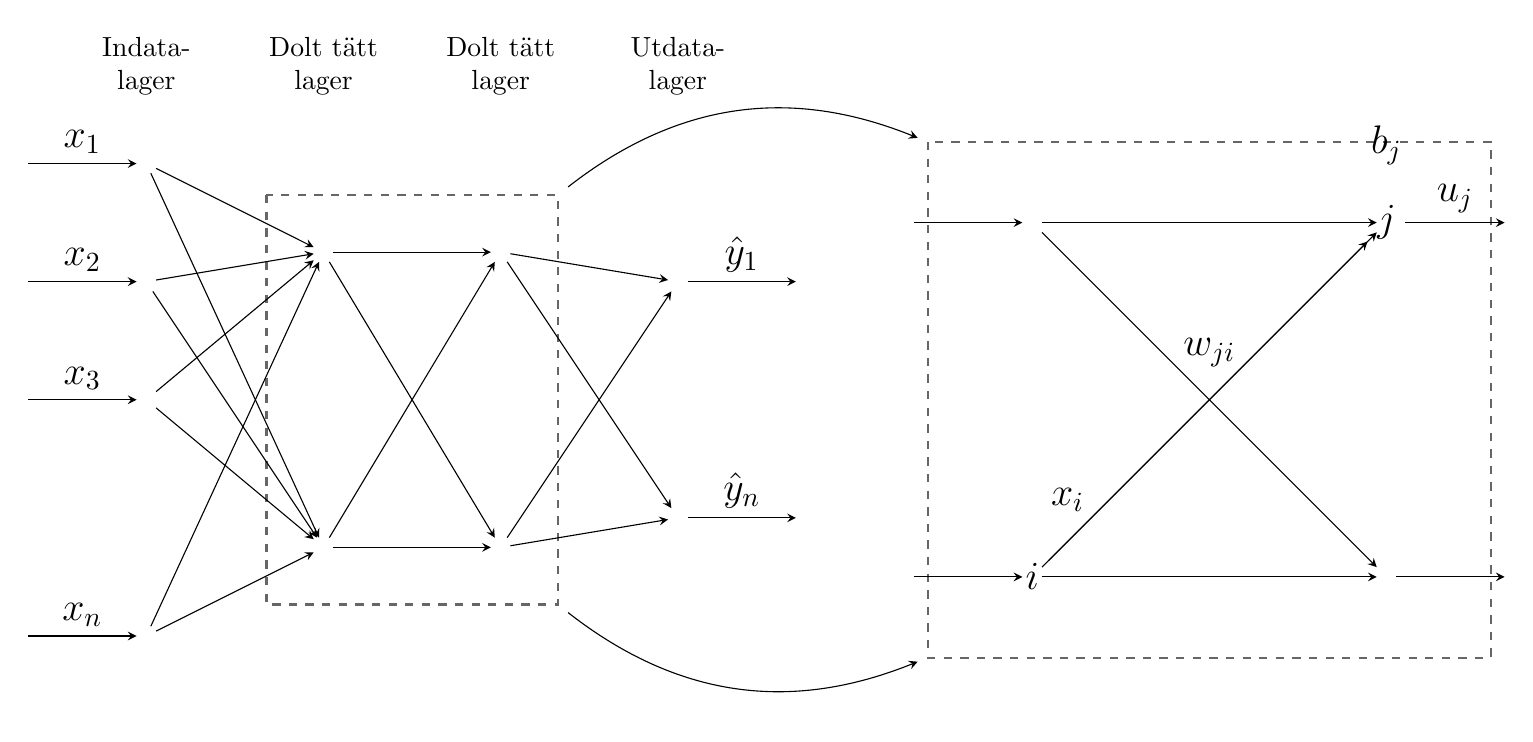
\begin{tikzpicture}[x=1.5cm, y=1.5cm, >=stealth]
\foreach \m/\l [count=\y] in {1,2,3,missing,4}
  \node [input neuron/.try, neuron \m/.try] (input-\m) at (0,2.5-\y) {};

\foreach \m [count=\y] in {1,missing,2}
  \node [dense neuron/.try, neuron \m/.try ] (hidden1-\m) at (1.5,2-\y*1.25) {};
  \foreach \m [count=\y] in {1,missing,2}
  \node [dense neuron/.try, neuron \m/.try ] (hidden2-\m) at (3,2-\y*1.25) {};

\foreach \m [count=\y] in {1,missing,2}
  \node [input neuron/.try, neuron \m/.try ] (output-\m) at (4.5,1.5-\y) {};

\foreach \l [count=\i] in {1,2,3,n}
  \draw [<-] (input-\i) -- ++(-1,0)
    node [above, midway] {\Large $x_\l$};

\foreach \l [count=\i] in {1,n}
  \draw [->] (output-\i) -- ++(1,0)
    node [above, midway] {\Large  $\hat{y}_\l$};

\foreach \i in {1,...,4}
  \foreach \j in {1,...,2}
    \draw [->] (input-\i) -- (hidden1-\j);
\foreach \i in {1,...,2}
  \foreach \j in {1,...,2}
    \draw [->] (hidden1-\i) -- (hidden2-\j);

\foreach \i in {1,...,2}
  \foreach \j in {1,...,2}
    \draw [->] (hidden2-\i) -- (output-\j);

\foreach \l [count=\x from 0] in {Indata-, Dolt tätt, Dolt tätt, Utdata-}
  \node [align=center, above] at (\x*1.5,2) {\l \\ lager};
  
  
% draw a box around zoom region

\draw[opacity=0.6, line width=0.3mm, dashed] ($(hidden1-1.north west)+(-0.4,0.4)$) rectangle ($(hidden2-2.south east)+(0.4,-0.4)$)
    node [] (box1) {}
    node (box2) at ($(hidden2-1.north east)+(+0.4,0.4)$)  {};



% ***** zoom

\foreach \m/\l [count=\y] in {1,2}
  \node [zoom neuron/.try, neuron \m/.try] (z_input-\m) at (7.5,5-\y*3-1) {};

\foreach \m [count=\y] in {1, 2}
  \node [zoom neuron/.try, neuron \m/.try ] (z_hidden1-\m) at (10.5,5-\y*3-1) {};


\foreach \l [count=\i] in {1,2}
  \draw [<-, zoom line/.try] (z_input-\i) -- ++(-1,0)
    node [above, midway] {};


\foreach \i in {1,...,2}
  \foreach \j in {1,...,2}
    \draw [->, zoom line/.try] (z_input-\i) -- (z_hidden1-\j);
    
% Mark certain nodes and corresponding lines
\node [highlight neuron/.try, neuron 1/.try ] (highlight-1) at (7.5,5-2*3-1) {\Large $i$};
\node [highlight neuron/.try, neuron 2/.try ] (highlight-2) at (10.5,5-1*3-1) {\Large $j$};
\node at (7.5+0.3,5-2*3-1+0.65) {\Large $x_{i}$};
\draw [->, highlight line/.try] (highlight-1) -- (highlight-2)
    node [] at (9, -0.1) {\Large $w_{ji}$};
\node at (10.5,5-1*3-1+0.65) {\Large $b_j$};
\draw [->, highlight line/.try] (highlight-2) -- ++(1,0)
    node [above, midway] {\Large $u_{j}$};
\draw [->, zoom line/.try] (z_hidden1-2) -- ++(1,0) {};

\draw[opacity=0.6, line width=0.25mm, dashed] ($(z_input-1.north west)+(-0.8,0.6)$) rectangle ($(z_hidden1-2.south east)+(0.8,-0.6)$)
    node (zoom1) at ($(z_input-2.south west)+(-0.8,-0.6)$) {}
    node (zoom2) at ($(z_input-1.north west)+(-0.8,0.6)$)  {};

% **** connect zoom and nn
\begin{scope}[->]
    \path[z_connect line/.try]
        (box1) edge[bend right] node [->, left] {} (zoom1)
        (box2) edge[bend left] node [->, left] {} (zoom2);
\end{scope}
\end{tikzpicture}

\end{document}